\chapter{Preliminaries and Necessary background}
\label{chapter:background}
In this chapter we present the necessary background and the already-investigated analysis done separately in graph kernels, random features, and maximum mean discrepancy. However, we show our analysis combining these different notions in one algorithm in the next chapter, so readers can skip this chapter in case they already have a strong footing in these topics.

\section{Necessary Notations}
Before introducing the aforementioned topics, we first introduce the necessary notations related to graph definition and graph kernels.
A graph of size n is by definition a pair $G=(V,E)$, where V is the set of the graph nodes (vertices) $V=\{v_1,...,v_n\}$, and $E\in V\times V$ is the set of edges between these nodes, i.e. $(v_i, v_j)\in E$ means that the graph has an edge from node $v_i$ to node $v_j$ (and vice versa since we consider undirected graphs in this work).
\newline $H=(V_H,E_H)$ is said to be a subgraph (graphlet) of G and we write $H\sqsubseteq G$, if and only if there exist an injective function $\mathcal{M}:V_H\xrightarrow{} V$ such that $(v,w)\in E_H \Leftrightarrow{(\mathcal{M}(v),\mathcal{M}(w))\in E}$.\newline
Any edge $(v_i, v_i)$ is called a self loop. In a general graph two vertices $v_i$ and $v_j$ may be connected by more than
one edge. A simple graph is a graph with no self loops
or multiple edges. Here we always consider simple graphs.\newline
A simple graph can equivalently be represented by an adjacency matrix $A$ of size $n \times n$. The $(i,j)-th$ entry of $A$ is 1 if an edge $(v_i, v_j)$ exists and zero otherwise.\newline
Two graphs $G=(V,E)$ and $G'=(V',E')$ are isomorphic and we write $G'\cong G$ if there exists a bijective function $\mathcal{M}:V\xrightarrow{} V'$ such that $(v_i,v_j)\in E$ iff $(\mathcal{M}(v_i),\mathcal{M}(v_j))\in E'$



\section{Graph Kernels}
In general, the kernel method is used to generate features for learning algorithms that is in its nature a function of the inner product of data points in the dataset (as in linear regression for instance). The mathematical basis behind it is that any positive definite function $\mathcal{K}(x,y)$ with $x,y \in \mathcal{R}^d$ defines an inner product and a lifting function $\phi$ so that the kernel value is equal to the inner product between lifted data points:
\begin{equation}
\label{eq:kernel_main_equation}
    \mathcal{K}(x,y) = <\phi(x),\phi(y)>
\end{equation}
The convenience one gets deploying kernels-based models is that there is no need to have the formula or the evaluations of the lifting function $\phi$. Instead, it is  sufficient to have the evaluations of the kernel itself $\mathcal{K}(x,y)$. To better illustrate this benefit, we take the Gaussian kernel as an example, where:
\begin{equation}
    \mathcal{K}_{G}(x,y)=exp(-\frac{\left \| x-y\right\|^2}{2\sigma^2})
\end{equation}
where $\sigma$ is called the bandwidth parameter of the kernel. The lifting function $\phi_G$ of this kernel is located in a Hilbert space of infinite dimension, but the kernel can be easily evaluated for any pair (x,y). 

\subsection{Graph kernels design}
Traditional kernel machines approach problems with vector-valued input data, where it compare different data points $(x,y \in \mathcal{R}^d)$ using the difference between correspondent pairs of vector entries. Based on that, these kernels are imperfect to be used with graphs, since the graph structure is permutation invariant, i.e. isomorphic graphs have different adjacency matrices but they represent the same structure. So in this case distance-kernels between graph representation vectors (adjacency matrices for example ) are uninformative. As a result it is necessary to measure distance between graphs in ways that are  permutation invariant as well. Here the concept of isomorphism is critical in learning algorithms on graphs,  not only because there is no known polynomial-time algorithm for testing graph isomorphism (except for graphs with specific structures), but isomorphism is also too strict for learning in a similar way to learning with equality operator \citep{kriege_graph_kernels}. \newline
Most of graph kernels developed for graph learning problems are convolution kernels, where given two graphs, the trick is to divide each into smaller subgraphs and then to pairwise compute the kernel between the resulted subgraphs.
\newtheorem{definition}{Definition} 
\begin{definition}[Convolution Kernel]
let $\mathcal{R}=\mathcal{R}_1\times...\times \mathcal{R}_d$ denote a space of components such that a composite object $X\in \mathcal{X}$ decomposes into elements of $\mathcal{R}$. Let $R:\mathcal{R}\xrightarrow{}\mathcal{X}$ denote the mapping from components to objects, such that $R(x)=X$ iff the components $x\in \mathcal{R}$ make up the object $X\in \mathcal{X}$, and let $R^{-1}(X)=\{x\in\mathcal{R}:R(x)=X\}$. then, the R-convolution kernel is:
\begin{equation}
\label{eq:conolutional_kernels}
    K_{CV}(X,Y)=\sum_{x\in R^{-1}(X)}~\sum_{y\in R^{-1}(Y)}~\underbrace{\prod_{i=1}^{d}k_i(x_i,y_i)}_{k(x,y)}
\end{equation}
with $k_i$ is a kernel on $\mathcal{R}$ for $i\in\{1,...,d\}$.
\end{definition}

 Applying this definition on graphs, $R^{-1}(G)$ includes all the components in graph $G$  that we want to compare with the components $R^{-1}(H)$ in graph $H$. One example of these kernels is the node label kernel, where for two graphs $G, H$, the mapping function $R$ maps the features $x_u\in \mathcal{R}$ of each node $u\in G\cup H$ to the graph that u is a member of. Another example that is mainly related to our work is the k-graphlet kernel, where $R$ here maps the subgraphs of size k to the graph in which it occur. The advantage of using convolution kernel framework with graphs is that kernels are permutation invariant on the graphs level as long as they are permutation invariant on the components level. 
 As a drawback, the sum in Eq.~\ref{eq:conolutional_kernels} iterates over every possible pair of components. As a result, when we choose our components to be more specific such that the kernel value is high between a component and itself while it is low between two different components, each graph becomes drastically similar to itself but distant from any other graph. Thus, a set of weights is usually added  so this problem is resolved.


\subsection{Graphlet Kernel}
\label{subsection: graphlet kernel}
Referring by $\mathcal{G}=\{graphlet(1),..., graphlet(N_k)\}$ to the set of all graphs of size $k$, we define for a graph $G$ the vector $f_G\in \mathcal{R}^{N_k}$, the i-th entry equals the normalized-number of occurrences of $graphlet(i)$ in G ($\#(graphlet(i)\sqsubseteq G)$). What should be noticed based on this definition is that no two different graphlets in $\mathcal{G}$ are isomorphic. $f_G$ is usually referred to by the k-spectrum of G, and this vector is the key idea behind graphlet kernel. 


\begin{definition}[Graphlet Kernel]
Given two graphs $G$ and $H$ of size $n_G,n_H \geq k$, the graphlet kernel $\mathcal{K}_g$ is defined as \citep{graphlet_kernel}:
\begin{equation}
\label{eq:graphlet_kernel}
    \mathcal{K}_g(G,H)=f_G^Tf_H.
\end{equation}
\end{definition}
Which naturally involves an associated Euclidean metric $d_\mathcal{K}(G,H) = \|f_G - f_{H}\|_2$.
The drawback of this kernel is that computing the k-spectrum vector costs huge computational time, as there are $\tbinom{n}{k}$  subgraphs of size $k$ in a graph G of size n. As a result, there is a trade off between a more accurate representation of the graph (larger value of k) and the computational cost. However, some techniques are used in order to resolve this limitation as sampling from graph technique (section \ref{graph_sampling}).

\subsection{Graph Sampling to approximate k-Graphlet Spectrum}
\label{graph_sampling}
The problem of Graph Sampling arises when we deal with a large-scale graph and the task is to pick a small-size sample subgraph/s that would be similar to the original graph with respect to some important properties.\newline
Sampling from graph techniques are used to resolve the processing cost limitation of graphlet kernel, and it can deployed in two different manners:
\begin{enumerate} \itemsep0pt \parskip0pt \parsep0pt
    \item directly sample $m$ sugraphs $\{H_1,...,H_m\}$ of size k, and then estimate the k-spectrum vector empirically:
    $f_G(i)=\frac{1}{m}\Sigma_{j=1}^m \mathbbm{1}[H_j=graphlet(i)]$
    \item sample m subgraphs  $\{H_1,...,H_m\}$ of size $n'$ such that $n\gg n'>k$, then estimate $f_G$ as follows:
    $f_G=\frac{1}{m}\Sigma_{j=1}^m f_{H_j}$, this method is usually being referred to by Mean Kernel Method and is used in problems with large-scale or random distribution-based infinity-size graphs (see \ref{subsec:MMD}).
\end{enumerate}  
The important thing here is whether a sufficiently large number of random samples will lead to an empirical k-spectrum vector close to the actual vector, and this is to be analyzed in chapter \ref{chapter:analysis}.

\section{Random Features}
Random features is a method developed to approximate kernel machines efficiently with a reasonable computational time. The idea is that instead of considering the true lifting function $\phi$ in Eq. \ref{eq:kernel_main_equation}, we explicitly map the data points to an Euclidean inner product space of low dimensionality. This mapping is done using an appropriate randomized feature map $z:\mathcal{R}^d \xrightarrow{}\mathcal{R}^D$. Then we approximate the kernel of two data points $x, y$ by the inner product of their random features:
\begin{equation}
\label{eq:approx_RF}
\mathcal{K}(x,y)=<\phi(x),\phi(y)> \approx z(x)^*z(y)
\end{equation}
Considering this approximation, we can transform the input with $z$ and then apply a fast linear learning method to have a similar learning power as the original non-linear kernel-based algorithm. \newline
The question here is how to construct $z$ for a specific kernel so that Eq. \ref{eq:approx_RF} is satisfied. In what follows, Random Fourier Features method to construct the random feature mapping function $z$ is presented.

\subsection{Random Fourier Features}
The following theorem represents the key idea behind this mapping method.
\newtheorem{theorem}{Theorem}
\begin{theorem}[Bochner's theorem]
A continuous and shift-invariant kernel $\mathcal{K}(x,y)=\mathcal{K}(x-y)$ on $\mathcal{R}^d$ is positive definite if and only if $\mathcal{K}(\delta)$ is the Fourier transform of a non-negative measure.
\end{theorem}
As a straight result, we can easily scale a shift-invariant kernel so that its Fourier transform $p(w)$ is a correct probability distribution, since it is non-negative measure and integral-bounded function, and we write:
\begin{equation}
\label{Fourier integral}
\mathcal{K}(x-y)=\int_{\mathcal{R}^d}p(w)e^{jw^T(x-y)}dw=E_w[e^{jw^Tx}{e^{jw^Ty}}^*]
\end{equation}
But both $p(w)$ and $\mathcal{K}(\delta)$ are real-valued functions, thus from Eq.~\ref{Fourier integral} we can prove that:
\begin{equation}
\label{real Fourier integral}
\mathcal{K}(x-y)=\int_{\mathcal{R}^d}p(w)cos({w^T(x-y)})dw=E_w[z_w(x)z_w(y)]
\end{equation}
where $z_w(x)=\sqrt{2}cos(w^Tx+b)$ such that $w$ is drawn from $p(w)$ and b is drawn uniformly from $[0,2\pi]$.\newline
As a result, $\ z_w(x)z_w(y)$ is an unbiased estimate of $\mathcal{K}(x,y)$. Moreover, we can achieve lower variance estimation to the expectation (Eq. \ref{real Fourier integral}) by averaging $m$ instances of the estimator with different random frequencies $w$. i.e. the low-variance estimator can be written as: $z(x)'z(y)=\frac{1}{m} \Sigma_{j=1}^m z_{w_j}(x)z_{w_j}(y)$. This estimator and based on Hoeffding's inequality guarantees exponentially fast convergence in $m$ between $z(x)'z(y)$ and the kernel true value:
\begin{equation}
    Pr(|z(x)'z(y)-\mathcal{K}(x,y)|\geq\epsilon)\leq2e^\frac{-m\epsilon^2}{4}
\end{equation}

\section{Random Projections with Optical Processing Units (OPU's)}
Random projections is one of the important techniques in machine learning and in signal processing. However, traditional random projection methods need a large memory to store the corresponding random matrix $W$ and a huge computational time to project the input data points $x$, i.e. to compute $Wx$. Optical processing units (OPU's) is the developed technology developed to solve the previous two drawbacks, where an OPU complete random projections at the speed of light without the need to store any random matrix. In general, Random projections are the result of two procedures where the first one is the linear-random projections and the second one is non-linear mapping.
Mathematically speaking, OPU's perform the following operation \citep{saade_opu}:
\begin{equation}
\label{OPU_equation}
    Y=\phi(WX+b);~W\in \mathcal{R}^{m\times d},b\in \mathcal{R}^m, U\in \mathcal{R}^d
\end{equation}
Where $b$ is a bias vector, $X$ is an input point, $m$ is the number of random features and $d$ is the input space dimension. Also, $W$ is a random i.i.d complex matrix with Gaussian real and imaginary parts and $\phi$ is the non-linear mapping function.\newline
In the limit where the number of random features $r\xrightarrow{}\infty$, it can be proven by the concentration of the measure that the inner product between the projected data points $(X_i\in \mathcal{R}^r)$ in the new feature space tends to a kernel function that depends only on the input points in the original feature space $(U_i\in \mathcal{R}^d)$

\subsection{OPU structure and functionality}
Eq.~\ref{OPU_equation} still imply that an OPU need to store and multiply by the random projection matrix. But in an OPU, a heterogeneous material, as a paper or any white translucid material, is used to scatter incident light in a very complex way. The behavior of the scattering process is considered random because of the extremely high complexity. One can argue that light scattering is a linear, deterministic, and reproducible phenomenon, but what can be said here is that the unpredictable behavior of the process makes it effectively a random process. That is why these materials are called opaque since all information embedded within the incident light is seemingly lost during the propagation through the material \citep{saade_opu}. An example used to demonstrate and justify the resulted randomness is a cube of edge length $100\mu m$, such cube can include $\approx 10^7$ paint nanoparticles, all the positions and shape of these particles must be known in order to predict its effect on light. Propagation through such a layer can be seen as a random walk because of frequent scattering with the nanoparticles, where light explores the whole volume and undergoes tens of thousands of such scattering steps before coming out from the other side in a few picoseconds.\newline

\begin{figure}[ht!]
\begin{center}
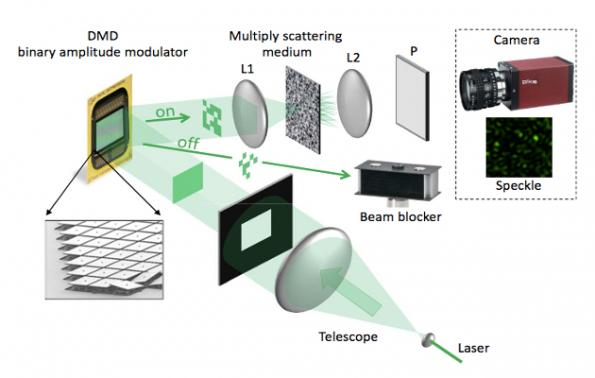
\includegraphics[scale=0.5]{figs/lighton630.jpg}
\end{center}
\caption[OPU's Experimental setup]{OPU's Experimental setup \citep{saade_opu}: A monochromatic laser is expanded by a telescope, then
illuminates a digital micromirror device (DMD), able to spatially encode digital information on the light beam by
amplitude modulation. The light beam carrying the signal is then focused on a random
medium by means of a lens. The transmitted light is collected on the
far side by a second lens, passes through a polarizer, and is measured by a standard monochrome CCD camera for example .}
\label{fig_opu}
\end{figure}
When the incident light is coherent, it promotes complex interference patterns, called speckles, due to the scattering process.
These speckles don't only characterize the propagation medium but also the incident light, and this can be modeled by $y=Wx$, 
where $y$ and $x$ are the vector amplitudes between a set of spatial modes at the output and at the input of the medium respectively. In OPUs, the transmission matrix $W$ of the propagation medium can be approximately considered as a Gaussian i.i.d matrix, it was also shown that even without $W$ being known, but it is guaranteed to be stable as long as the propagation medium is stable as a paint layer for instance \citep{saade_opu}.  So if we use a spatial light modulator and a laser to send an appropriate set of illuminations to the propagation medium, we can acquire the output intensity $|y|^2$ with a CCD or CMOS camera, and that is the principle concept behind OPU's functionality as seen in Fig~ \ref{fig_opu}.\newline 
The DMD (digital micromirror device) used in OPU's is a binary amplitude modulator consisting of an array of micro-mirrors, Each mirror can be lit or not, thus it can represent  a binary value. In order to represent grey values, each value is encoded on a square sub-array ($4\times 4$ for example) in the DMD, where the number of lit mirrors reflects the desired level of grey. DMD reflects the data and send the reflected light through the disordered medium, then a snapshot of the resulting random projection is acquired using a standard camera. all that is completed in a very high speed compared to the traditional random features techniques. 

\section{Mean kernel and Maximum Mean Discrepancy } \label{subsec:MMD}
The mean kernel methodology allows to \emph{lift} a kernel from a domain $\mathcal{X}$ to a kernel on \emph{probability distributions} on $\mathcal{X}$. Given a base kernel $k$ and two probability distribution $P,Q$, it is defined as
\begin{equation}\label{eq:mean_kernel}
\mathcal{K}(P,Q) = \mathbb{E}_{x \sim P, y \sim Q} \mathcal{K}(x,y)
\end{equation}
In other words, the mean kernel is just the expectation of the base kernel with respect to each term. The associated Euclidean metric is referred to by the  \emph{Maximum Mean Discrepancy (MMD)}, and is naturally defined as:
\begin{equation}\label{eq:MMD}
MMD(P,Q) = \sqrt{\mathcal{K}(P,P) + \mathcal{K}(Q,Q) - 2\mathcal{K}(P,Q)}
\end{equation}
It should be noticed here that $\mathcal{K}(P,P) = \mathbb{E}_{x \sim P, x' \sim P} \mathcal{K}(x,x') \neq \mathbb{E}_{x \sim P} \mathcal{K}(x,x)$.
